\documentclass[10pt,fleqn]{article} % Default font size and left-justified equations
\usepackage{import}
\usepackage[%
    pdftitle={SLCI : Transformée de Laplace},
    pdfauthor={Xavier Pessoles}]{hyperref}
\subimport{../../../../style/}{preambule}
%\fichetrue
\fichefalse

\proftrue
%\proffalse

\tdtrue
%\tdfalse

\courstrue
%\coursfalse

\subimport{../../../../style/}{new_style}
\subimport{../../../../style/}{macros_SII}
\subimport{../../../../style/}{preambule_trou}

\usepackage{siunitx}
% -------------------------------------
% Déclaration des titres
% -------------------------------------

\def\discipline{Enseignement \\Technologique \\ Transversal}
\def\xxtete{Enseignement Technologique Transversal}

\def\classe{1 STI2D}
\def\xxnumpartie{Séquence 2}
\def\xxpartie{Comparatif énergie pétrole et solaire}

\def\xxnumchapitre{Séance 2}
\def\xxchapitre{\hspace{.12cm} Énergies, Puissances et rendement}

\def\xxposongletx{2}
\def\xxposonglettext{1.45}
\def\xxposonglety{23}
\def\xxonglet{Seq. 2 -- TD 2}

\def\xxactivite{TD}
\def\xxauteur{\textsl{Geoffrey Vaquette}}

\def\xxcompetences{%
\textsl{%
\textbf{Savoirs et compétences :}
\begin{itemize}[label=\ding{112},font=\color{ocre}]
\item CO2.1	Identifier les flux et la forme de l'énergie, caractériser ses transformations et/ou modulations et estimer l'efficacité globale d'un système.
\end{itemize}
%
}}

\def\xxfigures{
\begin{center}

\includegraphics[height=4cm]{images/smartphone.png} \\
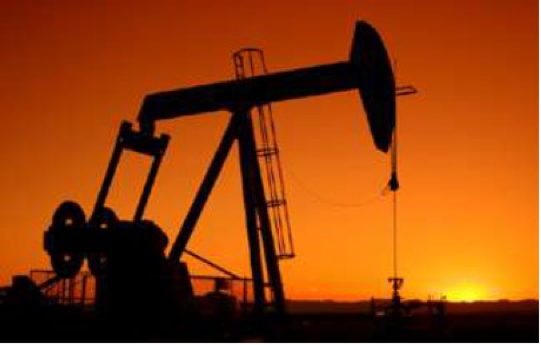
\includegraphics[height=4cm]{images/petrole.png} \\
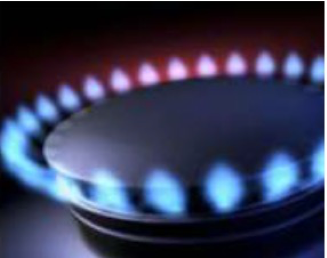
\includegraphics[height=4cm]{images/gaz.png} \\
\end{center}
}%figues de la page de garde
\def\xxpied{%
Energies, Puissances et Rendement \xxactivite%
}

%---------------------------------------------------------------------------

\renewcommand{\RemplirTrou}{true}
\begin{document}
\chapterimage{png/Fond_solaire}

\begin{obj}
Analyser et comparer les apports d’énergies de différentes sources. 

À travers cette activité, vous serez amené à comparer une source
d’énergie renouvelable et non renouvelable afin d’en faire ressortir les
avantages et inconvénients de chacune.
\end{obj}
\section{L'énergie pétrolière atteint ses limites}
 Environ 50 \% des réserves énergétiques mondiales de pétrole ont déjà
été pompées. Les réserves restantes connues sont estimées à \SI{164.4}{
\text{milliards de tonnes}}

\begin{exercise}
Une comparaison entre l'énergie solaire et le pétrole. 
%\begin{questions}
%\item 
\begin{question}
Sachant que la masse volumique moyenne du pétrole est
$\mu_p = \SI{0,8275}{kg/L}$, calculer le volume $V_p$ en litre de pétrole encore
disponible.
\end{question}

\begin{solution}
On a une masse $m_p = \SI{164.4e3}{MT}$ de pétrole. Connaissant la masse volumique du pétrole, on peut déduire : $$ m_p = \mu_p \times V_p \Rightarrow V_p = \frac{m_p}{\mu_p} = \frac{\num{164.4e3}\num{e6}\num{e3}}{0.8275} = \SI{1.98e14}{L} $$
\end{solution}

\begin{question}
Sachant que 1 baril de pétrole correspond à 159 litres ($V_{bl} = \SI{159}{L}$),
calculer le nombre de barils de pétrole $N_p$ encore disponibles.
\end{question}
\begin{solution}
$$N_p = \frac{V_p}{V_{bl}} = \frac{\num{1,98e14}}{159} = \SI{1,24e12}{bl}$$
Il reste \num{1,24e3} milliard de barils encore exploitables sur terre. 
\end{solution}
%\item 

\begin{question}
    Sachant que la consommation actuelle de pétrole est d’environ
80 Mbl/jour, calculer en combien de jour les réserves seront
épuisées. En déduire dans combien d’année il n’y aura plus de
pétrole au rythme actuel.
\end{question}
\begin{solution}
    Sachant que chaque jour on consomme \SI{80}{Mbl} et qu'il reste \SI{1,24e12}{bl} soit \SI{1,24e6}{Mbl}, on peut en déduire qu'à ce rythme, il restera du pétrole pour $$T = \frac{\num{1,24e6}}{\num{80}} = \SI{15550}{j} = \SI{43}{\text{années}}$$
\end{solution}

%\end{questions}
Une des sources d'énergie extérieures à la Terre et utilisable
actuellement est le soleil. Le soleil rayonne par an une énergie de
16.1015 kWh.

\begin{question}
    Combien faudrait-il de baril de pétrole pour avoir une énergie
équivalente. Comparer aux réserves restantes.
\end{question}

\begin{solution}
    Sachant que $\SI{1}{TEP} = \SI{11630}{kWh}$ correspond à l'énergie fournie par la combustion de 1 tonne de pétrole. Si on connaît la masse de pétrole, on pourra en déduire l'énergie encore exploitable.
    Connaissant le volume d'un baril $V_{bl} = \SI{159}{L}$ ainsi que la masse volumique du pétrole $\mu$, on peut déduire la masse d'un baril : $m_{bl} = \mu V_{bl} = 0,8275 \times \num{159} =  \SI{131,57}{kg}$). 
    
    On peut alors en déduire l'énergie encore exploitable : 
    $$E_p = \SI{131,57e-6}{TEP} = 11630\times \num{131,57e-6} = \SI{1,53}{kWh}$$
    
    Pour obtenir l'énergie équivalente au rayonnement du soleil, il faudrait donc : 
    $$Nb_{eq bl} = \frac{E_{\text{elec}}}{E_{bl}} = \frac{\num{16e15}}{\num{1,53e3}} = \SI{1,06e13}{barils}$$
\end{solution}
\end{exercise}

\section{Les centrales solaires seraient-elles une solution ?}
\begin{figure}[ht]
    \centering
    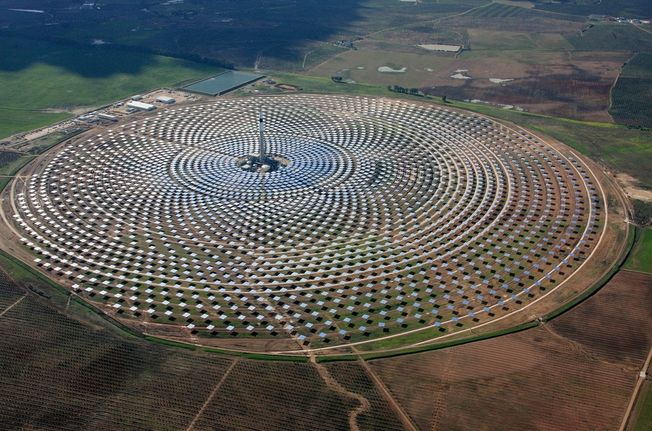
\includegraphics[width=0.4\textwidth]{images/Gemasolar.jpg}
    \caption{Centrale solaire Gemasolar en Espagne}
    \label{fig:gemasolar}
\end{figure}
Les panneaux solaires photo-voltaïques représentent
une solution de production d’énergie électrique à petite
échelle. Les centrales solaires à concentration
(chauffage d’eau par miroirs) permettraient une
production à plus grande échelle.
Pour vous faire une meilleure idée du potentiel de ces
centrales, vous allez calculer la surface nécessaire pour
produire la consommation mondiale d'électricité.
\pagebreak
\paragraph{Quelques chiffres : }
\begin{itemize}
    \item Production mondiale annuelle d'électricité : $E_\text{elec} = \SI{19000}{TWh}$
    \item Rendement net annuel sur toute la surface de la centrale : $\eta_c = \SI{14}{\%}$
    \item Puissance solaire en zone ensoleillée : $p_s = \SI{250}{W/m^2}$
    \item Rayon moyen de la Terre : $R = \SI{6371}{km}$
    \item Superficie totale de la Terre : $S = \SI{510072000}{km^2}$
    \item Proportion de terre ferme : $30\%$
\end{itemize}
\begin{exercise}
~
    \begin{question}
        L’énergie rayonnée par le soleil est-elle suffisante pour répondre à la demande énergétique mondiale annuelle d'électricité ?
    \end{question}
    
    \begin{solution}
        L’énergie rayonnée par le soleil (\SI{16.1015}{kWh}) est suffisante car elle est supérieure à la demande énergétique mondiale de \SI{19000}{Twh}.
    \end{solution}
    
    
    \begin{question}
        Calculer la puissance moyenne $P_m$ de la production mondiale
    \end{question}
    \begin{solution}
        On connaît l'énergie mondiale annuelle d'électricité : $E_\text{elec}$, on calcule la puissance moyenne à l'aide de la formule $E=P\times \Delta T$ : $$P = \frac{E}{\Delta T} = \frac{\num{19000e12}}{365\times 24} = \SI{2,16}{TW}$$
    \end{solution}
    \begin{question}
        En déduire la puissance moyenne Ps que doit fournir le soleil.
    \end{question}
    \begin{solution}
        Connaissant le rendement de la centrale ($\eta=\num{0,14}$) et la puissance désirée en sortie $P_s = \SI{2,16}{TW}$. A l'aide de la relation $\eta = \frac{P_s}{P_e}$, on peut écrire : 
        $$P_e = \frac{P_s}{\eta} = \frac{2,16e12}{0,14} = \SI{15,4}{TW}$$
    \end{solution}
    \begin{question}
        Quelle est la surface $S$ en \si{km^2} de centrale solaire nécessaire pour « capter » cette puissance ?
    \end{question}
    \begin{solution}
        Chaque \si{m^2} de terrain capte \SI{250}{W} de puissance solaire. Il faut donc $S_c = \frac{P_e}{p_s} = \frac{\num{15,4e12}}{250} = \SI{6,16e10}{m^2} = \SI{6,16e4}{km^2}$
    \end{solution}
    \begin{question}
        À quelle proportion de surface terrestre (sans les océans) de la terre cette surface correspond-elle ? 
    \end{question}
    \begin{solution}
        On calcule la surface hors océan $$S_T = 0,3 S = \SI{153021600}{km^2}$$
        On en déduit alors que $S_c$ représente $ \frac{S_c}{S_T} = \frac{61600}{153021600} = 0,0004 = 0,04\% $ 
    \end{solution}
    \begin{question}
        Comparer la surface de centrale solaire déterminée précédemment à un carré de \SI{250}{km} de côté. Le potentiel de ce type de centrale électrique peut-il subvenir aux besoins mondiaux en électricité ?
    \end{question}
    \begin{solution}
        Un carré de \SI{250}{km} de côté a une surface de \SI{62500}{km^2}, ce qui correspond à peu près à la surface de la centrale solaire qu’il faudrait pour subvenir à la production d’électricité annuelle mondiale. Cette surface étant assez faible par rapport à la surface totale de la Terre, on peut dire que ce type de centrale convient pour répondre au besoin d’électricité de la population mondiale.
    \end{solution}
    Voici une carte représentant la rentabilité de centrales solaires thermique sur terre. 
    \begin{center}
        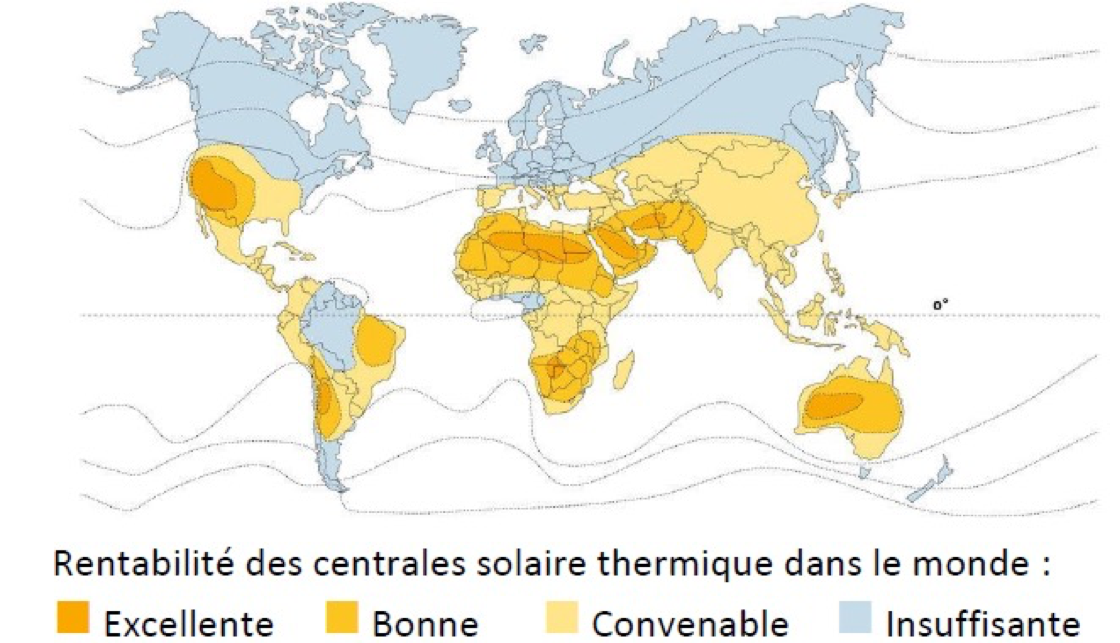
\includegraphics[width=0.8\textwidth]{images/carte_ensoleillement.png}
    \end{center}
    \begin{question}
        Au vu de la carte ci-dessus, quels arguments ne sont pas en faveur cette hypothèse ?
    \end{question}
    \begin{solution}
        On constate que, dans plusieurs zones, on pourrait installer la surface nécessaire pour produire l’électricité mondiale annuelle. Cependant, pour la moitié de la planète, l’ensoleillement est insuffisant, on ne pourrait donc pas installer ce type de centrale. Il faudrait ainsi transporter l’électricité produite dans les zones très ensoleillées vers les zones à faible ensoleillement, ce qui nécessiterait des installations importantes. Il est préférable, pour ces zones, de produire de l’électricité avec d’autres sources d’énergies comme l’énergie éolienne ou hydraulique. On peut donc dire que, en théorie, les centrales solaires suffiraient pour répondre au besoin en électricité de l’Homme mais en pratique, la mise en oeuvre est irréalisable.
    \end{solution}
    \begin{question}
        Réalisez une conclusion sur les apports énergétiques du soleil et du pétrole ainsi que sur les avantages et inconvénients de ces deux sources d’énergies. 
    \end{question}
    \begin{solution}
        On constate que le pétrole est une source d’énergie qui ne sera plus disponible d’ici peu de temps et que le soleil se trouve être une énergie qui pourrait prendre la relève car arrive sur terre en quantité suffisante.  
        
        Cependant, les centrales solaires ayant un rendement faible, elle ne peuvent pas être installée n'importe où sur Terre. Or, le déplacement de l'énergie électrique sur de très longues distances est complexe et rend donc impossible aujourd'hui l'exploitation exclusive de centrales solaires pour répondre aux besoins humains. 
        
        En comparaison, le pétrole (une fois extrait) se transporte relativement facilement (mais avec un impact environnemental non négligeable).
        
        En attendant que le rendement des centrales solaires soit nettement amélioré, l'utilisation d'autres énergies renouvelables comme les éoliennes ou les centrales hydrauliques est nécessaire pour s'affranchir du pétrole. 
    \end{solution}
\end{exercise}


\end{document}